% A partir da raiz, após gerar os resultados e a figura com os scripts R:
% latexmk -pdf -outdir=output/pdf model/plausibilidade_empirica_crossing_servicos.tex
\documentclass[11pt,a4paper]{article}
\usepackage[T1]{fontenc}
\usepackage[utf8]{inputenc}
\usepackage[brazilian]{babel}
\usepackage{lmodern,amsmath,amssymb,booktabs,graphicx,xcolor}
\usepackage[margin=2.45cm,top=2.2cm,bottom=2.2cm]{geometry}
\usepackage{caption,fancyhdr,hyperref}
\definecolor{tinta}{HTML}{172E3B}
\definecolor{azul}{HTML}{22576C}
\hypersetup{colorlinks=true,linkcolor=azul,urlcolor=azul,
 pdftitle={IA, trabalho relacional e poder coletivo},
 pdfsubject={A hipótese de Alex Imas e o alcance de um teste com dados setoriais}}
\captionsetup{font=small,labelfont=bf,labelsep=period,skip=4pt,hypcap=false}
\setlength{\parindent}{0pt}
\setlength{\parskip}{5pt plus 0.6pt minus 0.4pt}
\setlength{\headheight}{15pt}
\pagestyle{fancy}\fancyhf{}
\fancyhead[L]{\small\sffamily\color{azul}Mudança estrutural, organização do trabalho e democracia}
\fancyfoot[R]{\small\sffamily\thepage}
\renewcommand{\headrulewidth}{0pt}
\fancypagestyle{primeira}{\fancyhf{}\fancyfoot[R]{\small\sffamily\thepage}}
\newcommand{\titulo}[1]{\section*{\color{tinta}#1}}
\newcommand{\subtitulo}[1]{\par\smallskip{\large\bfseries\color{azul}#1\par}\nobreak}
\newcommand{\hubmer}{\href{https://www.econometricsociety.org/publications/econometrica/browse/2023/01/01/The-Race-Between-Preferences-and-Technology/supp/ecta200523-sup-0001-onlineappendix.pdf}{Hubmer (2023), suplemento, tabela B.I}}
\newcommand{\unionstats}{\href{https://unionstats.com/main.htm}{Hirsch, Macpherson e Even, Unionstats}}
\newcommand{\clm}{\href{https://dcomin.host.dartmouth.edu/Publications_files/ECTA16317.pdf}{Comin, Lashkari e Mestieri (2021)}}
\newcommand{\blsdoze}{\href{https://www.bls.gov/news.release/archives/union2_01232013.htm}{Bureau of Labor Statistics, 2012, tabela 3}}
\newcommand{\cornell}{\href{https://www.ilr.cornell.edu/faculty-and-research/labor-action-tracker-2025}{Cornell e University of Illinois, Labor Action Tracker 2025}}
\newcommand{\imasensaio}{\href{https://aleximas.substack.com/p/what-will-be-scarce}{Imas, \emph{What will be scarce?}}}
\newcommand{\imasnota}{\href{https://static1.squarespace.com/static/57967bc7cd0f68048126361d/t/69dbbeb4bd54b97b00d8dec3/1776008884067/Technical\%2BNote\%2BStructural\%2BChange.pdf}{nota técnica de Imas (2026)}}
\begin{document}
\thispagestyle{primeira}
{\small\sffamily\color{azul}Nota de pesquisa\hfill 23 de novembro de 2026\par}
\vspace{5pt}
{\LARGE\bfseries\color{tinta}IA, trabalho relacional e poder coletivo\par}
\vspace{5pt}

Um consultor pode usar IA para preparar um relatório e dedicar a hora que economizou a conversar com um cliente que conhece há anos. Ambas as tarefas são cognitivas. Na primeira, há evidência experimental de ganhos de produtividade na redação profissional. Na segunda, o cliente pode valorizar a atenção de alguém que sabe por que aquela decisão o preocupa. O consultor continua registrado na mesma ocupação e no mesmo ramo. Para a democracia, a questão é se essa mudança lhe dá, junto com outros trabalhadores, mais capacidade de agir coletivamente. \href{https://doi.org/10.1126/science.adh2586}{Noy e Zhang (2023).}

Alex Imas chama de \emph{relacional} a parte do que se compra cujo valor depende da participação humana, da autoria ou do vínculo com quem presta o serviço. Ele abre seu ensaio com o recado manuscrito do barista no copo de café. Uma máquina pode reproduzir as mesmas palavras. Saber que alguém as escreveu para aquele cliente pode integrar o que ele valoriza. Em sua nota técnica, Imas já aplica a demanda não homotética de Comin, Lashkari e Mestieri a esse mecanismo. Se a IA barateia a produção automatizável e a demanda relacional é relativamente mais sensível à renda, o ganho de poder de compra favorece a segunda. O efeito no emprego depende da intensidade de trabalho e dos salários relativos. \imasensaio{} e \imasnota.

\subtitulo{Quanto vale saber que alguém escreveu para mim?}
Em um experimento de campo aleatorizado em um varejista on-line, receber um bilhete manuscrito aumentou o gasto dos clientes que já eram fiéis à loja. Em outro estudo, as pessoas relataram menor disposição para recomendar uma empresa quando acreditavam que a IA tinha escrito uma mensagem emocional. Esse efeito foi menor quando a mensagem era factual ou quando a IA apenas revisava o texto. As duas pesquisas sustentam a ideia de que o cliente pode atribuir valor ao gesto humano. Resta estimar quanto a compra desse atributo cresce com a renda do cliente a preços comparáveis. Em Comin, Lashkari e Mestieri, os efeitos de renda explicam mais de 73\% da realocação de emprego \emph{dentro dos países prevista pelo modelo}, entre agricultura, manufatura e serviços. \href{https://doi.org/10.1177/10949968221102306}{Kim, Choi e Kim (2022)}, \href{https://doi.org/10.1016/j.jbusres.2024.114984}{Kirk e Givi (2025)} e \clm, p. 314.

\subtitulo{Quem se apropria do valor da relação?}
Se o toque pessoal fideliza o cliente à cafeteria, o ganho pode ficar com a rede. Se o cliente segue um profissional quando ele muda de firma, o vínculo pode dar poder de barganha ao trabalhador. Um estudo de assessores financeiros nos EUA estimou que, quando um acordo permitia a portabilidade, o assessor levava consigo cerca de 40\% dos ativos dos clientes ao trocar de firma. Os autores inferem esse limite inferior a partir dos ativos das firmas. O resultado documenta uma fonte de poder individual. Para proteger a competição eleitoral, esses trabalhadores precisariam também coordenar uma ação que o governante tivesse razões para levar em conta. \href{https://doi.org/10.1016/j.jfineco.2021.04.026}{Gurun, Stoffman e Yonker (2021), pp. 1219 e 1239.}

A pergunta que o modelo político precisa responder é se as pessoas cuja atenção se torna mais valiosa passam a ter \emph{juntas} mais capacidade de oposição. Um sindicato, por exemplo, pode reduzir o custo de coordenar uma paralisação. Em Buffalo, baristas e supervisores de turno de uma unidade da Starbucks elegeram representação sindical. A eleição mostra que pode haver organização nesse ambiente. O efeito de valorizar o toque pessoal sobre a organização continua em aberto. \href{https://www.nlrb.gov/case/03-RC-282115}{National Labor Relations Board, caso de Buffalo.}

\newpage
\titulo{1\quad Quando a atenção humana muda o resultado político?}
Partimos de uma democracia. Um governante ganha \(G>0\) ao restringir as eleições. Uma federação atribui valor \(V>0\) a preservá-las. Cada trabalhador do setor \(j\) pode produzir \(d_j\) unidades de oposição por unidade de esforço, que custa \(c_je^2/2\). A capacidade de oposição por trabalhador é \(b_j=d_j^2/c_j\). Se \(s\) é a parcela dos trabalhadores nos serviços relacionais \(S\), a federação consegue dissuadir o governante quando sua capacidade agregada \(M\) supera o limiar \(\tau\).
\[
 M=(1-s)b_A+s b_S > \tau,\qquad \tau=G^2/(2V).
\]
\(A\) é a atividade padronizável exposta ao choque de IA. Comparamos duas economias que partem dos mesmos empregos e enfrentam o mesmo choque, preços e instituições. Em \(H\), a preços constantes, as famílias gastam a renda adicional nas mesmas proporções de antes (demanda homotética). Em \(N\), dedicam uma parcela maior a serviços relacionais conforme enriquecem (demanda não homotética). Há um \textbf{\emph{crossing} político} quando as eleições se sustentam inicialmente, o governante as restringe em \(H\) e as preserva em \(N\). Isso requer
\[
 M_H(a)<\tau<\min\{M_0,M_N(a)\},
\]
onde \(a\) é o choque, medido pela fração de trabalho poupada por unidade na origem. Uma inversão local de sinal, \(M'_H(0)<0<M'_N(0)\), pode ocorrer longe do limiar. Para a decisão sobre as eleições, importam os níveis.

\subtitulo{O ganho ocorre entre postos de trabalho ou dentro da jornada?}
Se a demanda cria \textbf{postos relacionais adicionais}, seja \(s_N-s_H>0\) a diferença na parcela dos trabalhadores que chega a eles. Suponha que quem já trabalha nesses postos em \(H\) também o faça em \(N\) e mantenha sua capacidade, e que a origem conserve a mesma capacidade \(b_A(a)\) nos dois cenários. Denotando por \(b_{\mathrm{marg}}\) a capacidade média dos trabalhadores nos postos adicionais em \(N\), temos
\[
 M_N-M_H=(s_N-s_H)\,[b_{\mathrm{marg}}-b_A(a)].
\]
Para a realocação aumentar a capacidade de oposição, quem muda precisa ter mais capacidade no destino do que teria na origem. Para a realocação mudar a decisão do governante, esse ganho precisa ser suficiente para atravessar o limiar.

Se a IA \textbf{muda as tarefas no mesmo posto}, um assessor pode redigir menos relatórios e passar mais horas conversando com os clientes. O número de empregados fica constante. Nesse caso, o efeito no modelo passa pelo quanto cada um é substituível e pelo custo de agir com os colegas. Contar as horas de conversa como postos adicionais daria mais peso político à mesma pessoa por definição.

\subtitulo{O teste que identificaria o mecanismo}
Dentro de um mesmo serviço, observaríamos quanto se gasta para ter atendimento pessoal quando varia a renda do cliente, mantidas as opções e os preços relativos. Em seguida, verificaríamos quem ganha horas pagas ou é contratado, quem conserva o vínculo com o cliente e se os trabalhadores ganham meios de agir em conjunto. As medidas setoriais disponíveis nas páginas seguintes não observam essas margens. O \emph{crossing} para o mecanismo relacional de Imas permanece empiricamente em aberto.

\newpage
\titulo{2\quad O que se observa entre ramos de atividade}
Comparamos as elasticidades de gasto de 14 ramos americanos com a sindicalização de seus assalariados. Hubmer estima as elasticidades com a \emph{Consumer Expenditure Survey} de 1982--2012. A \emph{Current Population Survey} permite distinguir filiação e cobertura sindical. Mantemos as elasticidades históricas e variamos o ano dos dados do trabalho (2012, 2015 e 2025). As tabelas usam os valores antes do arredondamento, recuperados da replicação de Hubmer. \hubmer{} e \unionstats.

\begin{center}
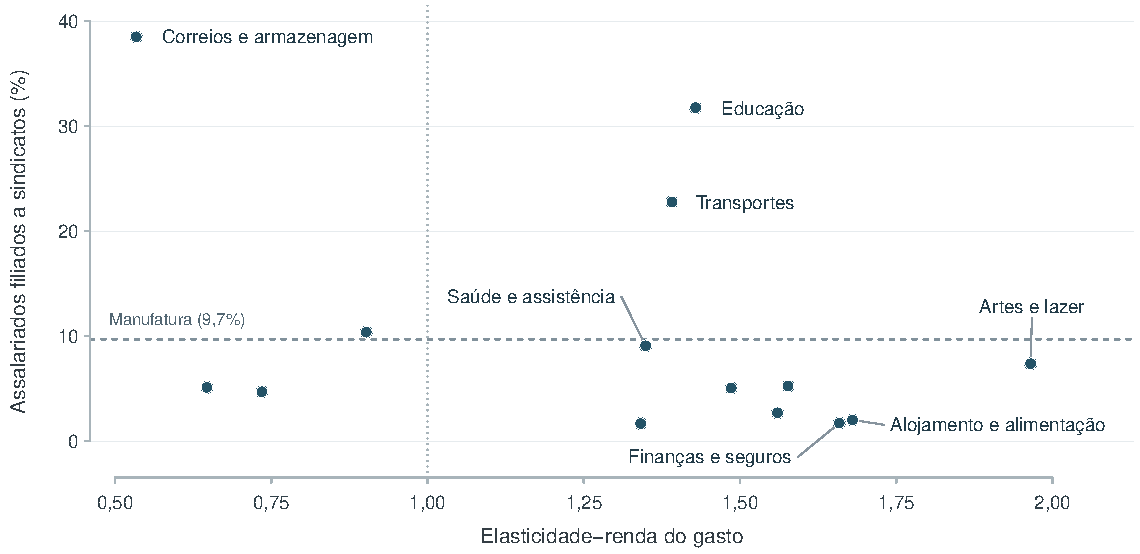
\includegraphics[width=.85\linewidth]{figures/elasticidade_sindical_servicos.pdf}
\captionof{figure}{Elasticidade de gasto e filiação sindical por ramo nos EUA. À direita de 1, o gasto no ramo aumenta mais do que o orçamento familiar. A linha horizontal marca a filiação na manufatura em 2012. Cada ponto mistura tarefas com diferentes graus de contato pessoal.}
\end{center}
\begin{center}
\captionof{table}{Associação entre a elasticidade de gasto e a fração dos assalariados filiados, nos mesmos 14 ramos dos EUA.}
\small\renewcommand{\arraystretch}{1.16}
\begin{tabular}{@{}lrrr@{}}\toprule
Como cada ramo entra na comparação & 2012 & 2015 & 2025 \\\midrule
Um voto por ramo, correlação de postos & \(-0{,}336\) & \(-0{,}393\) & \(-0{,}429\) \\
Peso no emprego, correlação de Pearson & \(-0{,}048\) & \(-0{,}027\) & \(-0{,}042\) \\
Peso no gasto de consumo, correlação de Pearson & \(-0{,}016\) & \(+0{,}019\) & \(-0{,}002\) \\\bottomrule
\end{tabular}
\end{center}
Retirando um ramo por vez, a correlação de postos de 2012 vai de \(-0{,}49\) a \(-0{,}17\). Usar cobertura por acordo no lugar de filiação também dá uma correlação negativa (\(-0{,}35\)). Quando damos mais peso aos ramos que empregam mais gente ou recebem mais gasto, a associação fica próxima de zero. Os coeficientes descrevem os ramos pareados e suas estimativas pontuais. A tabela não atribui a eles a precisão de uma amostra aleatória de indústrias.

Há uma leitura direta do resultado ponderado por gasto. Para cada dólar de consumo adicional, os ramos ganham parcelas proporcionais a \(w_j\gamma_j\), onde \(w_j\) é seu peso no consumo e \(\gamma_j\) sua elasticidade. Usando os pesos médios de gasto de 1982--2012 e a filiação de 2012, a taxa de filiação associada aos destinos desse dólar ficou apenas \textbf{0,03 ponto percentual abaixo} da taxa associada ao dólar médio. O cálculo é restrito aos serviços pareados e mantém preços e taxas sindicais fixos. Para saber quem ganha um \emph{emprego}, seria preciso ainda saber quantas horas de trabalho cada dólar de demanda requer.

\newpage
\titulo{3\quad Como os dados entram na calibração setorial}
No exercício entre ramos, supomos que o choque reduz a dependência do governante em relação aos trabalhadores que permanecem na origem, de modo que \(b_A(a)=(1-\rho a)^2\), com \(b_A(0)=1\). Tomamos a filiação ou a cobertura do setor, \(u_j\), como indicador observável de organização. Testamos \(b_S/b_A(0)=(u_S/u_A)^k\), com \(k=1\) e \(k=2\). O primeiro caso torna a capacidade proporcional à taxa. O segundo corresponde a eficácia \(d_j\) proporcional à taxa e custos de coordenação iguais. Essas são duas hipóteses sobre como converter organização em poder. Os dados de filiação, por si, admitem outras conversões. Mantemos \(\rho=0{,}50\) e \(\tau=20/9\) do esboço.

Para comparar dois ramos concretos, sejam \(\gamma_A\) e \(\gamma_S\) as elasticidades publicadas para a cesta inteira. Se \(s_0\) é a parcela inicial de \(S\) no par, o gasto do par cresce com elasticidade \((1-s_0)\gamma_A+s_0\gamma_S\). Logo a elasticidade de \(S\) em relação ao \emph{suborçamento do par}, ao longo da mesma variação de renda, é
\[
 \xi_{S\mid A,S}=\frac{\gamma_S}{(1-s_0)\gamma_A+s_0\gamma_S}.
\]
Trata-se de uma aproximação local para a economia de dois setores. Usamos tanto a parcela dos assalariados do par, sob a premissa do esboço de que gasto e emprego coincidem, quanto a parcela de gasto das contas de consumo pessoal. Assim, educação (\(1{,}429\)) ganha peso em relação à manufatura (\(0{,}731\)), mas perde peso em relação a finanças (\(1{,}659\)) quando a renda cresce a preços fixos. A escolha do setor exposto à IA altera a direção do canal.

Na demanda com elasticidade de substituição constante entre os dois setores, fixamos \(\eta=1\) em \(H\). Em \(N\), escolhemos \(\eta>0\) tal que \(\xi_{S\mid A,S}=\sigma+(1-\sigma)\eta/(1-s_0+s_0\eta)\). Após o choque, o equilíbrio entre produção e gasto determina \(s\) como a solução de
\[
 1-s=(1-s_0)(1-a)^{1-\sigma}(s/s_0)^{1/\eta}.
\]

A elasticidade de substituição entre os setores, \(\sigma\), vale 0,60 ou 0,20. Comin, Lashkari e Mestieri estimam 0,57 para três setores na amostra mundial e de 0,17 a 0,23 com habitação separada na amostra dos EUA. Testamos reduções do trabalho por unidade de 36\% e 13,04\%. O segundo valor equivale a produzir 15\% mais por hora, como no estudo de assistência por IA em atendimento ao cliente. Ele fornece uma referência de escala para uma atividade específica. \clm, tabelas III e XI, e \href{https://doi.org/10.1093/qje/qjae044}{Brynjolfsson, Li e Raymond (2025).}

\subtitulo{Quem emprega e quem negocia}
Na saúde e assistência, 9,1\% dos assalariados americanos eram sindicalizados em 2012, diante de 7,0\% nos estabelecimentos privados. Na educação, as taxas eram 31,7\% e 12,4\%. A expansão da provisão pública depende do financiamento por impostos e pode contratar trabalhadores com condições de negociação diferentes das de empregados privados. Isso importa quando se usam elasticidades do gasto familiar para prever quem vai se organizar. \blsdoze{} e \href{https://doi.org/10.1017/S0043887100007358}{Iversen e Wren (1998).}

A filiação também deixa parte da ação coletiva de fora. Em 2025, alojamento e alimentação liderou em \emph{número de paralisações} no levantamento de Cornell e Illinois. Foram em geral ações curtas, com poucos participantes. Saúde e assistência liderou em trabalhadores envolvidos e em dias de greve. As contagens também dependem do tamanho de cada ramo. Em outro estudo, Frymer, Grumbach e Hill estimam queda na qualidade da democracia eleitoral nos estados americanos que adotaram leis de \emph{right to work}, que restringem o financiamento sindical. Esse resultado sustenta a relevância política dos sindicatos. A estimativa estadual deixa em aberto quanto poder de oposição ganha um grupo específico de trabalhadores. \cornell{} e \href{https://doi.org/10.1017/S1537592724001427}{Frymer, Grumbach e Hill.}

\newpage
\titulo{4\quad Um exercício ilustrativo entre indústrias}
Usando só as elasticidades observadas e mantendo do esboço \(s_0=0{,}25\) e uma capacidade de oposição por trabalhador seis vezes maior no serviço do que na origem (\(b_S/b_A(0)=6\)), a decisão institucional se inverte em 10 dos 13 ramos compatíveis com essa especificação. O 14º, correios e armazenagem, tem elasticidade abaixo do domínio desse exercício. Ao usar também os contrastes sindicais, as elasticidades dos dois ramos e as parcelas observadas, o resultado muda.

\subtitulo{Manufatura e educação em 2015}
Com o limiar original \(\tau=2{,}2222\), esse é o único par e ano que produz a inversão direta entre as origens (manufatura ou finanças), os destinos e as conversões sindicais testadas. Foi por esse motivo que a educação apareceu no teste. A hipótese de Imas não confere primazia ao ramo. Na educação, 34,94\% dos assalariados eram cobertos por representação sindical. Na manufatura, 10,11\%. O caso positivo eleva a razão de cobertura ao quadrado, o que dá \(b_S=11{,}95\), e usa a parcela do \emph{gasto} do par, \(s_0=11{,}30\%\). A elasticidade educacional relativa ao orçamento do par é \(1{,}764\).

\begin{center}
\captionof{table}{Capacidade de defesa da competição eleitoral no par manufatura--educação. O governante mantém as regras quando a capacidade supera \(2{,}2222\).}
\small\renewcommand{\arraystretch}{1.16}\setlength{\tabcolsep}{4pt}
\begin{tabular}{@{}lrrrl@{}}\toprule
Choque e hipótese & Antes & Após, \(H\) & Após, \(N\) & Decisão após o choque\\\midrule
13,04\%, parcela no gasto & 2,238 & 2,189 & 2,314 & Só \(N\) preserva\\
36\%, parcela no gasto & 2,238 & 2,163 & 2,614 & Só \(N\) preserva\\
13,04\%, parcela no emprego & 6,228 & 6,317 & 6,444 & Ambos preservam\\
13,04\%, gasto e novos postos privados & 2,238 & 2,135 & 2,153 & Ambos restringem\\\bottomrule
\end{tabular}
\end{center}
{\small Cobertura de 2015, conversão quadrática, \(\rho=0{,}50\) e \(\sigma=0{,}60\). As duas elasticidades de gasto são comuns a todas as linhas.}

Com a parcela no \emph{emprego} de 47,74\%, já há trabalhadores organizados em número suficiente para dissuadir o governante nos dois cenários. Com \(\sigma=0{,}20\) e o peso de gasto, o efeito de preços já preserva a competição em ambos. Com filiação ao quadrado ou cobertura linear e o peso de gasto, a dissuasão inicial já falha. Na especificação que cruza, a capacidade inicial supera o limiar por apenas 0,69\% de seu valor. Os pontos estimados de gasto e organização não incorporam incerteza amostral neste exercício.

\subtitulo{A condição específica desse par}
Mantivemos os trabalhadores que já estavam na educação com sua cobertura de 34,94\%. Só aos postos adicionais atribuímos a taxa de 15,8\% observada na educação privada em 2015. A última linha da Tabela 2 mostra que ambos os cenários passam a restringir as eleições. Com o choque menor, a inversão ocorre se a cobertura dos \emph{novos} postos ficar entre 25,84\% e 42,54\%. Abaixo do piso, a mobilização é insuficiente mesmo em \(N\). Acima do teto, já basta em \(H\). Com o choque maior, os limites são 23,32\% e 39,17\%. São exigências do modelo que dados sobre as contratações induzidas pela renda poderiam confrontar. \href{https://www.bls.gov/news.release/archives/union2_01282016.htm}{Bureau of Labor Statistics, 2015, tabela 3.}

Os dados também permitem comparar finanças e seguros com alojamento e alimentação. Em 2012, suas elasticidades de gasto eram praticamente iguais (1,66 e 1,68) e a filiação era baixa nos dois ramos (1,71\% e 2,01\%). Usando a parcela no emprego e a filiação, tanto a conversão linear quanto a quadrática já colocam a capacidade inicial abaixo do limiar. Falta a condição inicial para que esse par ilustre a preservação de uma democracia que antes dissuadia o governante. Finanças inclui conversas de aconselhamento, e alimentação inclui tanto preparo padronizado quanto atenção pessoal. Essas médias deixam indeterminada a elasticidade do toque pessoal nas duas atividades.

\vfill
{\footnotesize Fontes consultadas em 23/11/2026. Os dados originais, as tabelas de cálculo e a revisão independente acompanham esta nota no repositório do projeto.}
\end{document}
